% AER E 361 Mission Report Template
% Spring 2023
% Template created by Yiqi Liang and Professor Matthew Nelson

% Document Configuration DO NOT CHANGE
\documentclass[12 pt]{report}
% --------------------LaTeX Packages---------------------------------
% The following are packages that are used in this report.
% DO NOT CHANGE ANY OF THE FOLLOWING OR YOUR REPORT WILL NOT COMPILE
% -------------------------------------------------------------------

\usepackage{hyperref}
\usepackage{parskip}
\usepackage{titlesec}
\usepackage{titling}
\usepackage{graphicx}
\usepackage{graphviz}
\usepackage[T1]{fontenc}
\usepackage{titlesec, blindtext, color} %for LessIsMore style
\usepackage{tcolorbox} %for references box
\usepackage[hmargin=1in,vmargin=1in]{geometry} % use 1 inch margins
\usepackage{float}
\usepackage{tikz}
\usepackage{svg} % Allows for SVG Vector graphics
\usepackage{textcomp, gensymb} %for degree symbol
\hypersetup{
	colorlinks=true,
	linkcolor=blue,
	urlcolor=cyan,
}
\usepackage{biblatex}
\addbibresource{main.bib}
\usepackage{amsmath}
\usepackage{listings}
\usepackage{multicol}
\usepackage{array}

\usepackage{hologo} %KYR: for \BibTeX
%\usepackage{algpseudocode}
%\usepackage{algorithm}
% This configures items for code listings in the document
\usepackage{xcolor}

\usepackage{fancyhdr} % Headers/Footers
\usepackage{siunitx} % SI units
\usepackage{csquotes} % Display Quote
\usepackage{microtype} % Better line breaks

\definecolor{commentsColor}{rgb}{0.497495, 0.497587, 0.497464}
\definecolor{keywordsColor}{rgb}{0.000000, 0.000000, 0.635294}
\definecolor{stringColor}{rgb}{0.558215, 0.000000, 0.135316}
\definecolor{mygreen}{rgb}{0,0.6,0}
\definecolor{mygray}{rgb}{0.5,0.5,0.5}
\definecolor{mymauve}{rgb}{0.58,0,0.82}

\lstdefinestyle{customc}{
  belowcaptionskip=1\baselineskip,
  breaklines=true,
  frame=L,
  xleftmargin=\parindent,
  language=C,
  showstringspaces=false,
  basicstyle=\footnotesize\ttfamily,
  keywordstyle=\bfseries\color{green!40!black},
  commentstyle=\itshape\color{purple!40!black},
  identifierstyle=\color{blue},
  stringstyle=\color{orange},
 }

 \lstset{ %
  backgroundcolor=\color{white},   % choose the background color; you must add \usepackage{color} or \usepackage{xcolor}
  basicstyle=\footnotesize,        % the size of the fonts that are used for the code
  breakatwhitespace=false,         % sets if automatic breaks should only happen at whitespace
  breaklines=true,                 % sets automatic line breaking
  captionpos=b,                    % sets the caption-position to bottom
  commentstyle=\color{commentsColor}\textit,    % comment style
  deletekeywords={...},            % if you want to delete keywords from the given language
  escapeinside={\%*}{*)},          % if you want to add LaTeX within your code
  extendedchars=true,              % lets you use non-ASCII characters; for 8-bits encodings only, does not work with UTF-8
  frame=tb,	                   	   % adds a frame around the code
  keepspaces=true,                 % keeps spaces in text, useful for keeping indentation of code (possibly needs columns=flexible)
  keywordstyle=\color{keywordsColor}\bfseries,       % keyword style
  language=Python,                 % the language of the code (can be overrided per snippet)
  otherkeywords={*,...},           % if you want to add more keywords to the set
  numbers=left,                    % where to put the line-numbers; possible values are (none, left, right)
  numbersep=8pt,                   % how far the line-numbers are from the code
  numberstyle=\tiny\color{commentsColor}, % the style that is used for the line-numbers
  rulecolor=\color{black},         % if not set, the frame-color may be changed on line-breaks within not-black text (e.g. comments (green here))
  showspaces=false,                % show spaces everywhere adding particular underscores; it overrides 'showstringspaces'
  showstringspaces=false,          % underline spaces within strings only
  showtabs=false,                  % show tabs within strings adding particular underscores
  stepnumber=1,                    % the step between two line-numbers. If it's 1, each line will be numbered
  stringstyle=\color{stringColor}, % string literal style
  tabsize=2,	                   % sets default tabsize to 2 spaces
  title=\lstname,                  % show the filename of files included with \lstinputlisting; also try caption instead of title
  columns=fixed                    % Using fixed column width (for e.g. nice alignment)
}

\lstdefinestyle{customasm}{
  belowcaptionskip=1\baselineskip,
  frame=L,
  xleftmargin=\parindent,
  language=[x86masm]Assembler,
  basicstyle=\footnotesize\ttfamily,
  commentstyle=\itshape\color{purple!40!black},
}

\lstset{escapechar=@,style=customc}

\titlelabel{\thetitle.\quad}

% From here on out you can start editing your document
\newcommand{\subtitle}[1]{%
  \posttitle{%
    \par\end{center}
    \begin{center}\LARGE#1\end{center}
    \vskip0.5em}%
}

\title{\textbf{Iowa State University
\\{\Large Aerospace Engineering}}}
\subtitle{AER E 322 Lab 8\\
		  Thin-Walled Section and Shear Center}
\author{Matthew Mehrtens, Peter Mikolitis, and Natsuki Oda}

\newcommand{\etal}{\textit{et al}., }
\newcommand{\ie}{\textit{i}.\textit{e}., }
\newcommand{\eg}{\textit{e}.\textit{g}., }

% Define the headers and footers
\setlength{\headheight}{70.63135pt}
\geometry{head=70.63135pt, includehead=true, includefoot=true}
\fancypagestyle{plain}{
	\fancyhead{}\fancyfoot{} % clears the headers/footers
	\fancyhead[L]{\textbf{AER E 322}}
	\fancyhead[C]{\textbf{Aerospace Structures Laboratory Report}\\
					 \textbf{Lab 8 Thin-Walled Section and Shear Center}\\
					 Section 4 Group 2\\
					 Matthew Mehrtens, Peter Mikolitis, and Natsuki Oda\\
					 \today}
	\fancyhead[R]{\textbf{Spring 2023}}
	\fancyfoot[C]{\thepage}
}
\pagestyle{fancy}
\fancyhead{}\fancyfoot{} % clears the headers/footers
\fancyhead[L]{\textbf{AER E 322}}
\fancyhead[C]{\textbf{Aerospace Structures Laboratory Report}\\
			  \textbf{Lab 8 Thin-Walled Section and Shear Center}\\
			  Section 4 Group 2\\
			  Matthew Mehrtens, Peter Mikolitis, and Natsuki Oda\\
			  \today}
\fancyhead[R]{\textbf{Spring 2023}}
\fancyfoot[C]{\thepage}

\begin{document}
\maketitle
\tableofcontents

\chapter{Pre-Lab} \label{pre-lab}
\section{Introduction} \label{introduction}
To reduce the weight and cost of aircraft, aerospace engineers use thin-walled structures throughout aerostructures, particularly in the wings. In addition to being more weight and cost effective than traditional structures, they are generally equally strong. Unfortunately, one of the side effects of thin-walled structures is their tendency to twist under unsymmetrical loadings.

To evaluate the strength of thin-walled structures, we have to determine where the shear center is, \ie the point where applied loads bend and do not twist the structure. In this lab, we learned how to calculate the shear center and deflection of a thin-walled structure.

\section{Objectives} \label{objectives}
Using the five provided specimens, we will apply twisting loads to thin-walled beams and make a number of measurements for each specimen. We will use the material learned in lecture and in the lecture notes to calculate the shear center of the thin-walled beams. 

\section{Hypothesis} \label{hypothesis}
Although our individual results from prelab varied significantly from each other, we expect the actual shear center values to at least correlate to the answers we calculated in prelab, even if they are off by a constant or a proportionate. We predict the cross sectional and the angle of opening will have a significant impact on the materials shear center and resistance or tendency to twist.

\chapter{Lab Work} \label{lab_work}
\section{Variables} \label{variables}
\subsection{Independent Variables} \label{variables-independent_variables}
\begin{itemize}
	\item Weight of mass; the applied load varied amongst the specimens
	\item Material of the specimen; the material of the element affects the local stiffness or strength and its tendency to twist
	\item Cross-section of the specimen; this variable controls the value of I which is used to derive the location of the shear center 
\end{itemize}

\subsection{Dependent Variables} \label{variables-dependent_variables}
\begin{itemize}
	\item Deflection due to load; these deflections take the form of bending as observed in cantilevered beams or torsional deflections in the form of twist 
	\item Shear center; the point about which applied loads cause bending but not torsion. The shear center is dependent on the cross-sectional layout. 
\end{itemize}

\section{Work Assignments} \label{work_assignments}
Refer to Table \ref{table:work_assignments} for the distribution of work during this lab.

\begin{table}[!htbp]
\caption{Work assignments for AER E 322 Lab 8.}
\begin{center}
	\begin{tabular}{| c | c | c | c |}
		\hline
		\multicolumn{1}{| c |}{\textbf{Task}} & \textbf{Matthew} & \textbf{Peter} & \textbf{Natsuki} \\
		\hline
		\multicolumn{4}{| c |}{\textit{Lab Work}} \\
		\hline
		Date Recording & X & X & X \\
		\hline
		Exp. Setup & X & X & X \\
		\hline
		Exp. Work & X & X & X \\
		\hline
		Exp. Clean-Up & X & X & X \\
		\hline
		\multicolumn{4}{| c |}{\textit{Report}} \\
		\hline
		Introduction & X & & X \\
		\hline
		Objectives & & & X \\
		\hline
		Hypothesis & X & & X \\
		\hline
		Variables & & X & \\
		\hline
		Materials & & X & \\
		\hline
		Apparatus & & X & \\
		\hline
		Procedures & & X & \\
		\hline
		Data & & & \\
		\hline
		Analysis & X & X & X \\
		\hline
		Conclusion & X & X & \\
		\hline
		References & X & & \\
		\hline
		Appendix & X & & \\
		\hline
		Revisions & X & X & \\
		\hline
		Editing & X & & \\
		\hline
	\end{tabular}
\end{center}
\label{table:work_assignments}
\end{table}

\section{Materials} \label{materials}
\begin{itemize}
	\item Five beam specimens as described in Table \ref{tbl:specimens}
	\item \qty{100}{\g} and \qty{200}{\g} mass
	\item Ruler
	\item Clamp; to secure one end of the beams
	\item Level
\end{itemize}

\begin{table}[!htbp]
\caption{Dimensions and specifications for the five different specimens.}
\begin{center}
	\begin{tabular}{|c|c|c|c|c|c|c|}
		\hline
		Specimen &Cross section &Height, &Width, &Thickness, &Outer &Opening \\
		ID&type&$h$ (\unit{inch})&$b$ (\unit{inch})&$t$ (\unit{inch})&diameter, &angle, \\
		&&&&&$OD$ (\unit{inch})&$2\theta_0$ (\unit{deg})\\
		\hline
		I&Plastic C-channel&2.43&1.456&0.08&N/A&N/A\\
		\hline
		II&Metal C-channel&0.84&0.56&0.055&N/A&N/A\\
		\hline
		III&PVC circular open&N/A&N/A&0.071&1.66&3.1\\
		\hline
		IV&PVC circular open&N/A&N/A&0.071&1.66&36.3\\
		\hline
		V&PVC circular open&N/A&N/A&0.071&1.66&103.7\\
		\hline
	\end{tabular}
\end{center}
\label{tbl:specimens}
\end{table}

\section{Apparatus} \label{apparatus}
The five beams should be cantilevered with the clamp. On the free end, there is a cross beam on which the weight will be hung. Figure \ref{fig:cbar} shows the apparatus for the C-channel beam and Figure \ref{fig:pvcbar} shows the apparatus for the circular PVC beam.

\begin{figure}[htbp]
	\centering
	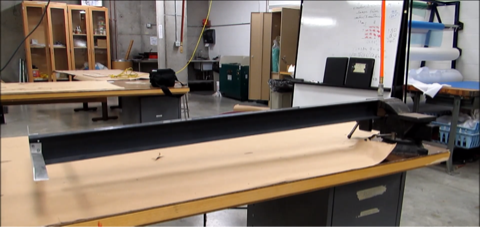
\includegraphics[width=6in]{images/c-channel beam}
	\caption{One of the cantilevered C-channel beams from lab eight \cite{demo_video}.}
	\label{fig:cbar}
\end{figure}
\begin{figure}[htbp]
	\centering
	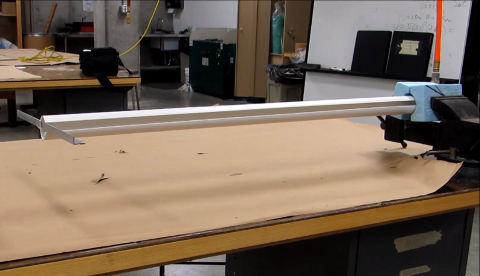
\includegraphics[width=6in]{images/circular pvc beam}
	\caption{One of the cantilevered circular PVC beams from lab eight \cite{demo_video}.}
	\label{fig:pvcbar}
\end{figure}

\section{Procedures} \label{procedures}
Set up the five beams as described and shown in Section \ref{apparatus}. Ensure the beams and the table are level. For specimen one, perform a preliminary measurement: measure the length from the edge of the clamp to the cross bar and measure the height from the table to a reference point at the same length as the cross bar, \eg the bottom of the beam.

For each of the five beams, perform the following procedure at least four times---placing the weight at least twice on each side of the cross beam:
\begin{enumerate}
	\item Level the cross bar as best you can. For the circular specimens, this can be done by rotating the beam. Measure the height at both ends of the cross bar to calculate the initial angle of twist. For specimens one and two, if the initial angle of twist is greater than \qty{1}{\degree}, account for this baseline by subtracting the initial angle of twist from subsequent angle of twist calculations.
	\item Place a weight on the cross beam at an arbitrary location (at least twice on both sides). Use the \qty{100}{\g} weight for specimens one, three, and five, and use the \qty{200}{\g} weight for specimens two and four.
	\item Record the location of the weight along the cross bar and the height of both sides of the cross beam. Since the shear center is measured from the center of the circular beams and from the center of the vertical web of the C-beams, make sure to note where your cross beam measurements are referenced from. Later in the analysis you can adjust your cross beam measurements to be relative to the shear center.
\end{enumerate}

For specimen one, put the weight at the shear center, \ie the point where an applied weight causes no twist, and measure the height at the reference point again. This should give you beam deflection.

\section{Data} \label{data}
\textbf{Note:} Our group misinterpreted the lab instructions for this lab. Instead of measuring the height of the cross beam at both ends, we measured the height of the actual beam at both ends. The numbers we calculated in lab are, of course, meaningless. After looking through the lab instruction more closely, it is obvious we were supposed to measure the height of the cross beam to calculate the angle of twist.

To still be able to do the analysis properly, we asked a fellow group in our AER E 322 section, Section \num{4} Group \num{3}, if we could use their data. They agreed; all data used in this report is courtesy of lab group \num{3} in AER E 322 section \num{4}.

To calculate angle of twist, we used Equation \ref{eqn:aot} from the lab eight lecture notes \cite{lecture_notes}:
\begin{align} \label{eqn:aot}
	\theta&=\sin^{-1}\left(\frac{h_R-h_L}{L}\right)
\end{align}
where $h_R$ is the height from the table to the right end of the cross bar, $h_L$ is the height from the table to the left end of the cross bar, and $L$ is the length of the cross bar. Figure \ref{fig:aot} shows this angle visually.

\begin{figure}[htbp]
	\centering
	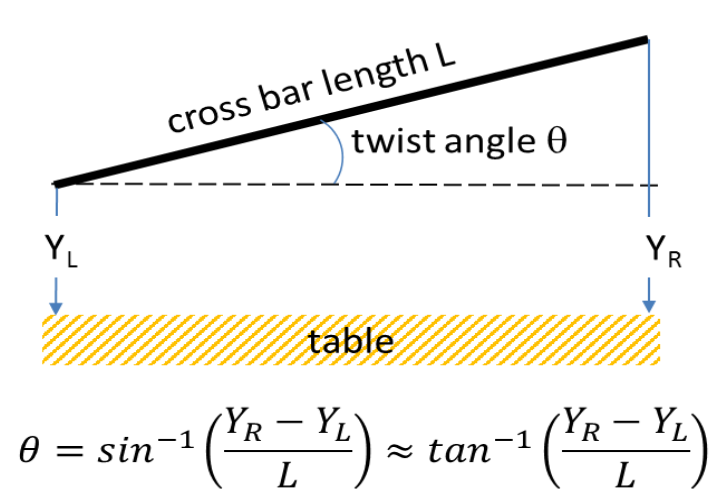
\includegraphics[width=4in]{images/aot}
	\caption{Visual representation of the angle of twist of the cross bar. \cite{lecture_notes}}
	\label{fig:aot}
\end{figure}

The data we used in the analysis portion of this lab is shown in Table \ref{tbl:data}.

\begin{table}[!htbp]
\caption{Data collected from lab eight, courtesy of lab group \num{3} from AER E 322 section \num{4}. $h$ is the height of the cross bar at the left and right ends, $L$ is the length of the cross bar, $\theta$ is the angle of twist, calculated using Equation \ref{eqn:aot}, $x$ is the distance to the weight on the cross bar, and $m$ is the mass of the weight.}
\begin{center}
	\begin{tabular}{|c|c|c|c|c|c|c|c|}
		\hline
		Specimen&$h_L$ (\unit{\cm})&$h_R$ (\unit{\cm})&$L$ (\unit{\cm})&$\theta$ (\unit{\degree})&$x_L$ (\unit{cm})&$x_R$ (\unit{cm})&$m$ (\unit{\g})\\
		\hline
		\num{1}&\num{10.4}&\num{13.1}&\num{44.0}&\num{3.52}&\num{11.0}&N/A&\num{100}\\
		\hline
		\num{1}&\num{8.8}&\num{14.6}&\num{44.0}&\num{7.57}&\num{14.0}&N/A&\num{100}\\
		\hline
		\num{1}&\num{17.7}&\num{4.8}&\num{44.0}&\num{-17.0}&N/A&\num{9.2}&\num{100}\\
		\hline
		\num{1}&\num{18.7}&\num{3.4}&\num{44.0}&\num{-20.3}&N/A&\num{12.8}&\num{100}\\
		\hline
		\num{2}&\num{9.9}&\num{11.4}&\num{30.0}&\num{2.87}&\num{3.1}&N/A&\num{200}\\
		\hline
		\num{2}&\num{8.1}&\num{13.0}&\num{30.0}&\num{9.40}&\num{9.0}&N/A&\num{200}\\
		\hline
		\num{2}&\num{11.6}&\num{9.5}&\num{30.0}&\num{-4.01}&N/A&\num{3.3}&\num{200}\\
		\hline
		\num{2}&\num{12.6}&\num{8.3}&\num{30.0}&\num{-8.24}&N/A&\num{7.5}&\num{200}\\
		\hline
		\num{3}&\num{7.7}&\num{12.5}&\num{30.0}&\num{9.21}&\num{4.9}&N/A&\num{100}\\
		\hline
		\num{3}&\num{6.9}&\num{13.4}&\num{30.0}&\num{12.5}&\num{7.4}&N/A&\num{100}\\
		\hline
		\num{3}&\num{12.1}&\num{8.2}&\num{30.0}&\num{-7.47}&N/A&\num{9.8}&\num{100}\\
		\hline
		\num{3}&\num{11.5}&\num{9.1}&\num{30.0}&\num{-4.59}&N/A&\num{5.6}&\num{100}\\
		\hline
		\num{4}&\num{9.8}&\num{13.4}&\num{30.0}&\num{6.89}&\num{5.0}&N/A&\num{200}\\
		\hline
		\num{4}&\num{8.9}&\num{14.7}&\num{30.0}&\num{11.1}&\num{7.6}&N/A&\num{200}\\
		\hline
		\num{4}&\num{15.3}&\num{6.1}&\num{30.0}&\num{-17.9}&N/A&\num{7.5}&\num{200}\\
		\hline
		\num{4}&\num{14.2}&\num{7.7}&\num{30.0}&\num{-12.5}&N/A&\num{4.5}&\num{200}\\
		\hline
		\num{5}&\num{10.0}&\num{13.8}&\num{30.5}&\num{7.16}&\num{4.5}&N/A&\num{100}\\
		\hline
		\num{5}&\num{7.6}&\num{16.4}&\num{30.5}&\num{16.8}&\num{10.8}&N/A&\num{100}\\
		\hline
		\num{5}&\num{15.0}&\num{7.2}&\num{30.5}&\num{-14.8}&N/A&\num{5.6}&\num{100}\\
		\hline
		\num{5}&\num{17.2}&\num{5.8}&\num{30.5}&\num{-21.9}&N/A&\num{10.6}&\num{100}\\
		\hline
	\end{tabular}
\end{center}
\label{tbl:data}
\end{table}

\chapter{Conclusion} \label{conclusion-chapter}
\section{Analysis} \label{analysis}
\subsection{Problem 1}
The measured shear centers and the theoretical shear center are shown in Table \ref{tbl:shear_centers}.

\begin{table}[!htbp]
\caption{Dimensions and specifications for the five different specimens.}
\begin{center}
	\begin{tabular}{|c|c|c|c|}
		\hline
		Specimen&$e_\text{meas}$ (\unit{cm})&$e_\text{theor}$  (\unit{cm})&Error (\unit{\percent})\\
		\hline
		1&\num{-0.800}&\num{-1.48}&\num{45.8}\\
		\hline
		2&\num{-0.322}&\num{-0.590}&\num{45.4}\\
		\hline
		3&\num{0.798}&\num{-4.03}&\num{119.8}\\
		\hline
		4&\num{-3.77}&\num{-3.87}&\num{2.79}\\
		\hline
		5&\num{-3.52}&\num{-3.21}&\num{9.54}\\
		\hline
	\end{tabular}
\end{center}
\label{tbl:shear_centers}
\end{table}

% TODO: Add analysis of problem 1

Take out outlier, error drops to 103.113% for specimen 3

\subsection{Problem 2}
First, we calculate the beam deflection theoretically using the method of superposition. Specifically, we refer to the max deflection formula, Equation \ref{eqn:deflection}, for a cantilevered beam shown on slide \num{14} of the week seven lecture notes \cite{week_7_lecture_notes}.
\begin{align}\label{eqn:deflection}
	\nu_\text{max}&=\frac{-PL^3}{3EI}
\end{align}
where $\nu_\text{max}$ is the maximum deflection of the beam, $P$ is the applied load, $L$ is the length of the beam, $E$ is the Young's Modulus, and $I$ is the moment of inertia. Substituting the proper values for this specimen, we find that
\begin{align*}
	\nu_\text{max}&=\frac{-(\qty{0.100}{\kg})(\qty{9.81}{\m\per\s\squared})(\qty{1.10}{\m})^3}{(\qty{3e9}{\Pa})(\qty{1.792e-7}{\m^4})}\\
	&=\qty{-2.43}{\mm}
\end{align*}
In lab, we measured the deflection to be $\qty{15.0}{\cm}-\qty{15.2}{\cm}=\qty{-0.2}{\cm}=\qty{-2}{\mm}$. This very closely matches the theoretical calculation, the limiting factor being the ruler we used to measure the height.

\subsection{Problem 3}
% TODO: Revise

We will use Figure \ref{fig:cross_sections} from the lab eight instructions \cite{lab_instructions} as a visual guide to our shear flow derivations.

\begin{figure}[htbp]
	\centering
	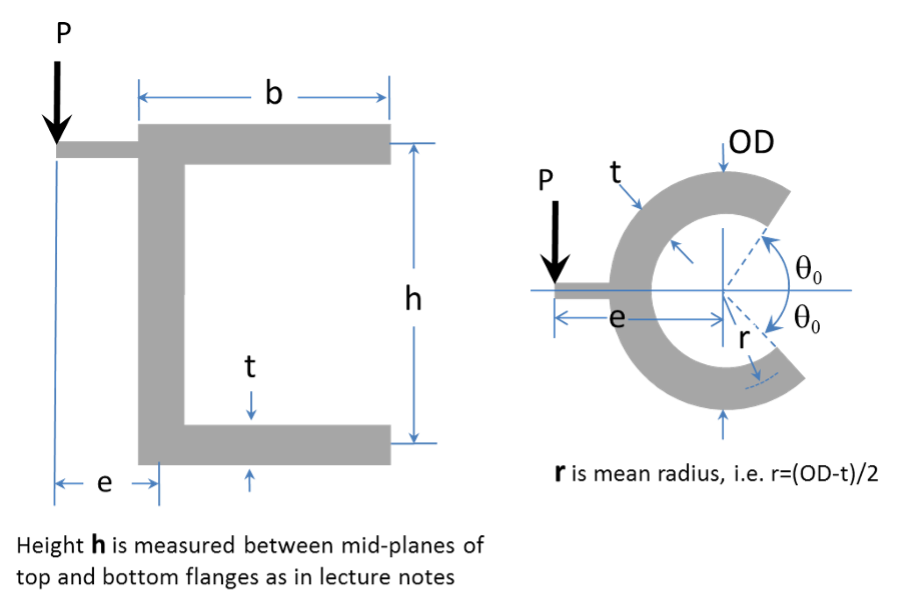
\includegraphics[width=4in]{images/cross sections}
	\caption{Schematic diagrams of the thin-walled cross section of the specimen: (left) C-channel and (right) circular open channel.}
	\label{fig:cross_sections}
\end{figure}

See Figure \ref{fig:peter_work} for our shear flow calculations.

\begin{figure}[htbp]
	\centering
	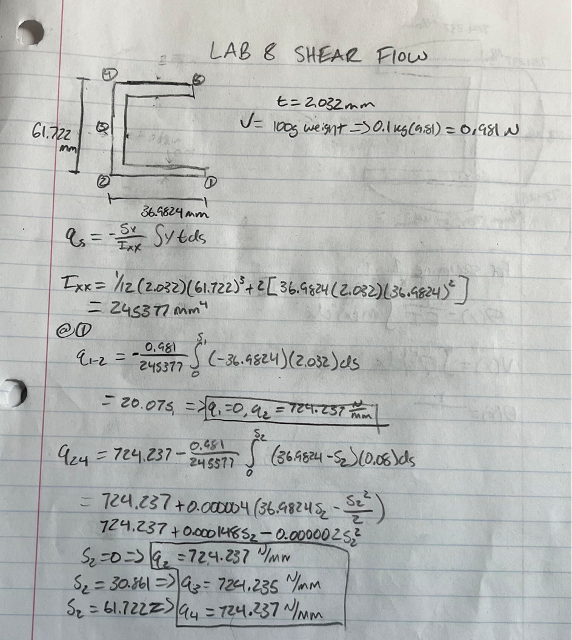
\includegraphics[width=6in]{images/peter shear flow}
	\caption{Calculation of shear flow in specimens one and two.}
	\label{fig:peter_work}
\end{figure}

\subsection{Problem 4}\label{problem_4}
% TODO: Revise

\begin{align*}
	\text{Specimen }\num{1}\text{: }(x,y)&=(\num{10.787},\num{0}) \unit{\mm}\\
	\text{Specimen }\num{2}\text{: }(x,y)&=(\num{3.507},\num{0}) \unit{\mm}
\end{align*}
Since the cross section is symmetrical across the $y$-axis, we know that the $y$-coordinate for shear center will be \num{0} due to the placement of the $x$-axis being at $\frac{h}{2}$. Then we can find the $x$-coordinate by using the equation for e above.  

\subsection{Problem 5}
% TODO: Revise

If the height increased significantly, the sample would be more comparable to a rectangular beam. Since $h$ would increase so much, $h$ would dominate the equation making $b$ insignificant. Above the equation used to calculate $I$ as for that of a C-section, but since can be cut out, the new equation for $I$ would be that of a rectangular beam. Substituting our derived $I$ equation into the $e$ equation, we see that as $h$ approaches infinity, $e$ approaches \num{0}. This would offset the shear center to be at the origin used in question \ref{problem_4}. Because the load of offset slightly, there will still be an angle of twist in the part, but due to the same reason stated earlier, the angle of twist would be so small it would extremely small.

\subsection{Problem 6}
% TODO: Revise

During the increase of both opening angle and radius, shape of the section going not to look like $C$. Increasing open angle, the open portion gets itself bigger. If the open angle reaches \qty{180}{\degree} ($2\theta_0=\qty{180}{\degree}$), shape of cross section will look like the circular pipe split in half along to path of that. However, the area value of this section will be bigger, depending on the value of increment. The equation below expresses the area of section with the circular given:
\begin{align*}
	A&=\pi\left(r+\frac{t}{2}\right)^2\frac{360-2\theta_0}{360}-\pi\left(r-\frac{t}{2}\right)^2\frac{360-2\theta_0}{360}
\end{align*}
The area will increase depending on how the value of the open-angle and radius increase. That is because the radius increases quadratically. But after open angle reaches \qty{90}{\degree}, the value will start to decrease because shear center will approach radius.

\begin{figure}[htbp]
	\centering
	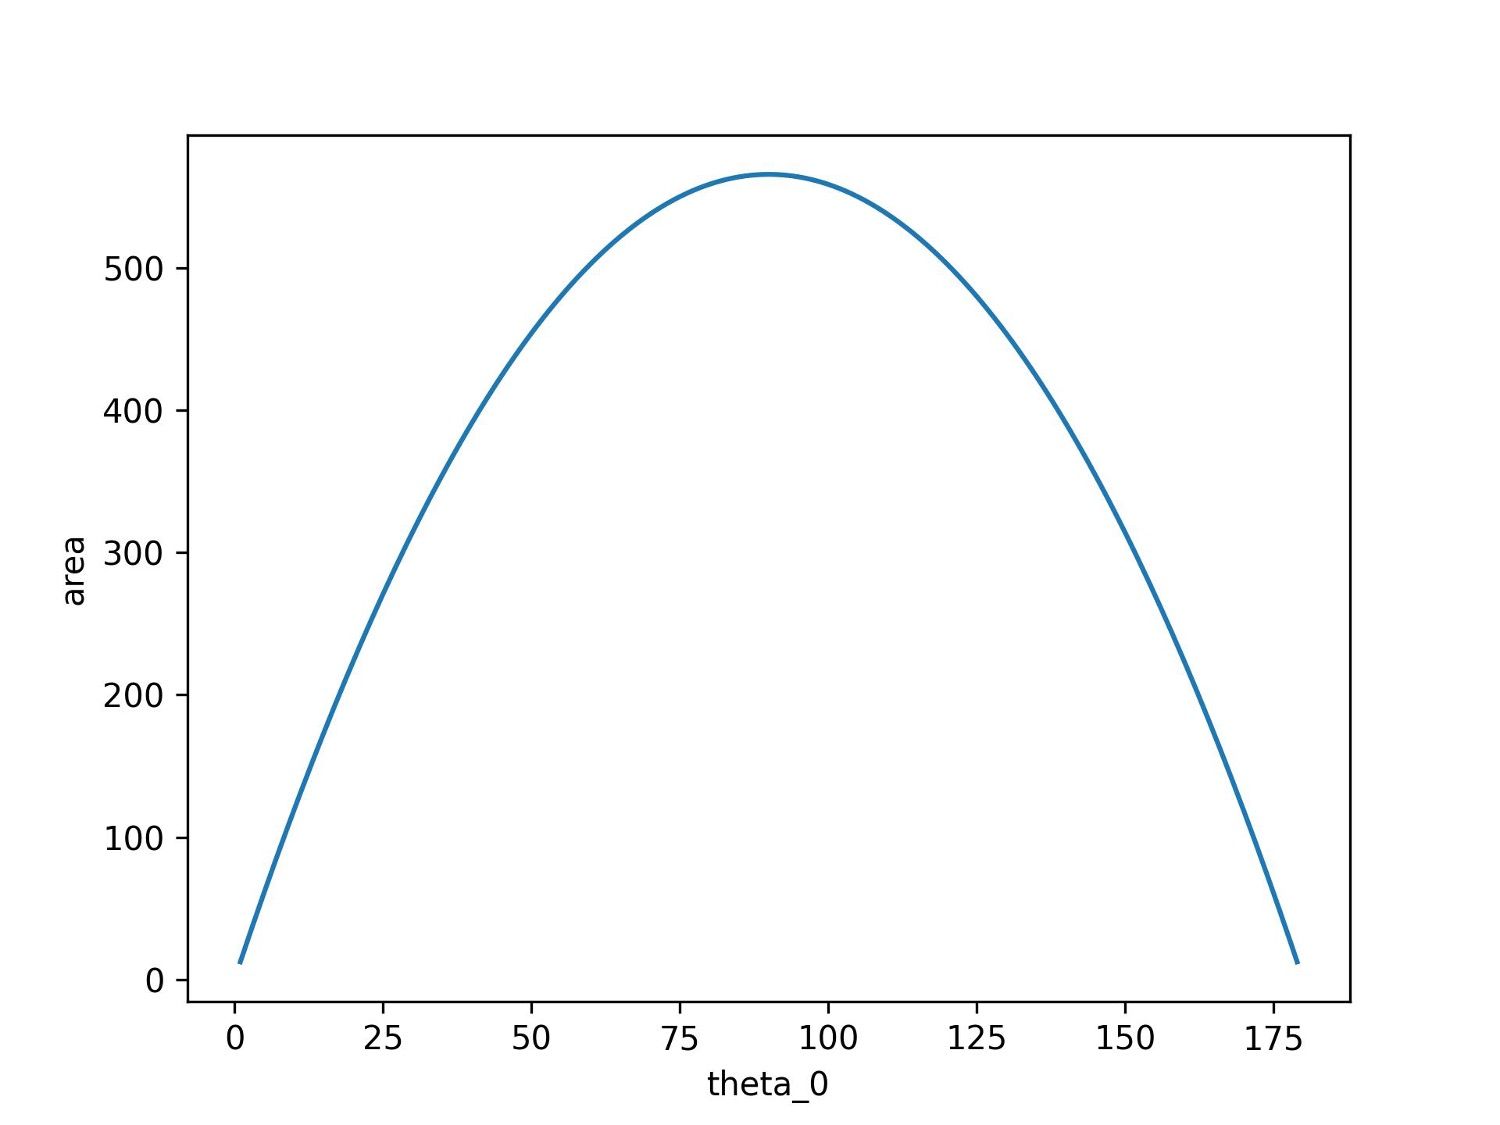
\includegraphics[width=4in]{images/Graphs/random_graph}
	\caption{The changes when both radius and degree of open angle increases one by one.}
	\label{fig:random_graph}
\end{figure}

\section{Sources of Error}\label{sources_of_error}
The most significant source of error in this lab is likely our own derivations and calculations. Known of our theoretical shear value calculations in the prelab agreed and none of our prelab values matched the measured shear centers. To accurately calculate the relative error between the theoretical and measured shear centers, we will need to revisit our derivations and calculations.

Additionally, many of the typical sources of error still apply. If the lab table or the beam was not initially level, all our measurements would be systematically incorrect. If the thickness of the beams or the dimensions were not exactly as described in the lab instructions, this would also result in higher error. Since we were measuring by hand, there is a possibly for random human error to propagate through our calculations due to the inconsistent way in which we measure things visually.

\section{Conclusion} \label{conclusion-section}
% TODO: Revise

Overall, our theoretical values did not match our measured values. This is mainly due to poor derivations or calculations, as described in Section \ref{sources_of_error}. Each group member had differing derivations for these specimens. Although our derivations were incorrect, we could provide valuable insights into how the material would react under load. The measured values that were obtained proved to be reliable data for finding the actual shear centers of each specimen.

\printbibliography[heading=subbibintoc]
\appendix
\end{document}
